\chapter{Work Breakdown Structure}

The work breakdown structure(WBS) describes which activities and tasks SitaWare Civilian is expected to have. This will give a better overview of the system, and thereby a better guess of a timetable.

\begin{figure}[H]
\centering
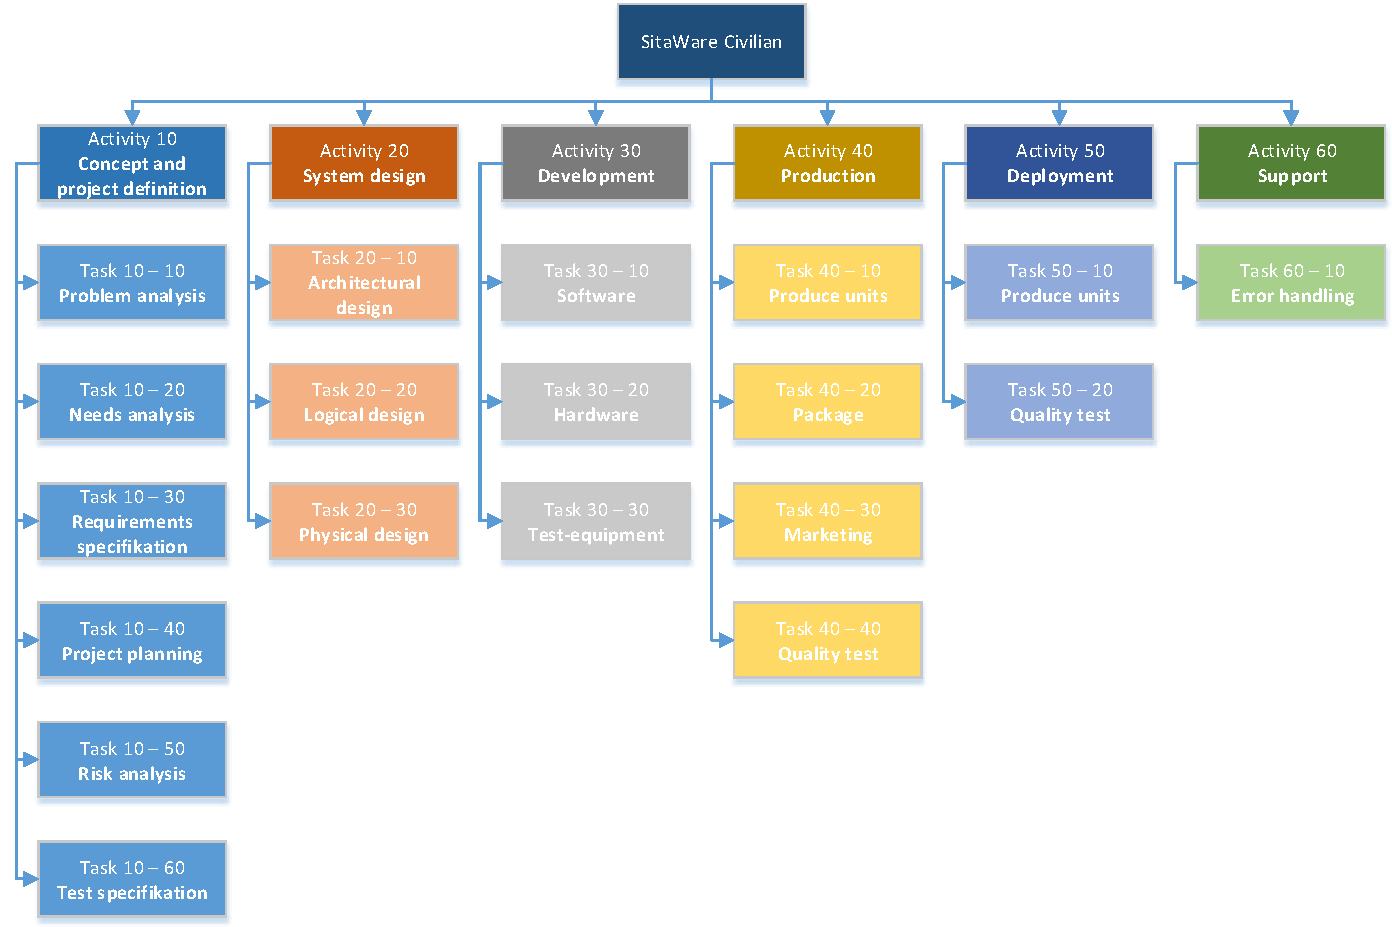
\includegraphics[width=0.95\textwidth]
{Billeder/WBS/WBS_v1.0.pdf}
\caption{Work Breakdown Structure.}
\label{fig:WBS}
\end{figure}

The activities in the WBS is based on the project phases. The tasks is a base for the timetable.

\begin{table}[H]
\begin{tabular}{|l|l|p{9cm}|}
\hline
\textbf{Reference} & \textbf{Taskname} & \textbf{Description} \\ \hline
10 - 10 & Problem analysis & Description and analysis of the main problem. 
\\  \hline
10 - 20 & Needs analysis & Description and analysis of the needs that will solve the main problem. 
\\  \hline
10 - 30 & Requirements specification & Description and analysis of the requirements of the system to solve the needs. 
\\  \hline 
10 - 40 & Test specification & Description of how to test the requirements.
\\  \hline
20 - 10 & Project planning & Description and planning of the major system phases.
\\  \hline 
20 - 20 & Risk analysis & Description and analysis of risks of the project.
\\ \hline
10 - 10 & Problem analysis & Description and analysis of the main problem. 
\\  \hline
10 - 20 & Needs analysis & Description and analysis of the needs that will solve the main problem. 
\\  \hline
10 - 30 & Requirements specification & Description and analysis of the requirements of the system to solve the needs. 
\\  \hline 
10 - 40 & Project planning & Description and planning of the major system phases.
\\  \hline 
\end{tabular}
\caption{Description of quality methods.}
\end{table}